\chapter{High-resolution Imaging of 3C295}

% % % % % % % % % % % % % % % % % % % % % % %
\section{Aims \& Methodology}
\pg
Our aim in this section is to create a high-resolution model of 3C295, something that - as
of yet - does not exist. More specifically, we seek to create a model that will allow us to find
good phase-calibration solutions for LOFAR international baselines. While we also solve for
amplitude gains, we know that we will need to correct the total source flux in each frequency
subband as our initial spectral model is not necessarily correct.
We select 6 sub-bands out of the total LOFAR HBA bandwidth, evenly spread throughout the bandwidth as shown in Fig. \ref{fig.freqsamp}.

\pg
This approach should allow us to appropriately constrain the final spectral behaviour of our high-resolution model, once the amplitude correction is applied to ensure our model is compliant with pre-existing flux measurements for this source \citepads{arse}. [put image of source flux as function of frequency for 3c295, citing source and ideally showing position of our subbands]

\pg
Our procedure is as follows: we self-calibrate individual subbands, starting from a model
extracted from a high-resolution VLA observation of 3C295 at 8.7 GHz \citepads[cf.][]{1991AJ....101.1623P}. Once this is done,
we extract and apply a scalar flux correction factor for each subband so that the integrated flux of our 3C295 image is compatible with the existing literature at all frequencies. The resulting model is then reliable enough to calibrate our Groth Strip data using the full LOFAR array and the entire HBA bandwidth.

% % % % % % % % % % % % % % % % % % % % % % %
\section{Data Reduction}

\subsection{Data \& Observation Properties}
\pg
The dataset used for this PhD project is part of the LOFAR Surveys KSP Tier-1 survey, which consists of a number of 8-hour pointing covering as much of the sky visibile to LOFAR as possible. We analyse one of these pointings, an observation performed on the 28th of August 2014 and centred on the Extended Groth Strip. As part of the Tier-1 survey, it is an 8-hour-long observation. We limit ourselves to analysing only the HBA observation, meaning that we use 365 sub-bands which sample a total bandwidth of [give bandwidth]. We use all Core and Remote LOFAR stations, as well as some of the International stations which were online at the time (specifically the German stations 1-5 and 7, along with the Swedish and the British station).

\pg
The data was acquired through the LOFAR Long-Term Archive, and is thus pre-processed and flagged for RFI using the standard tools ([cite aoflagger, ndppp?]). 

\subsection{Calibrating the Data}
\pg
Since we plan on applying an amplitude correction based on the works of Scaife \& Heald \citep[see][]{arse}, our overriding concern is to find good phase and amplitude gain without concern for the overall scaling factor. As such, our calibration strategy consists of calibrating 6 subbands, chosen across the LOFAR bandwidth, simultaneously. The chosen subbands, and their position in the total bandwidth, are shown here:
\begin{figure}[h]
\begin{floatrow}
\ffigbox{%
  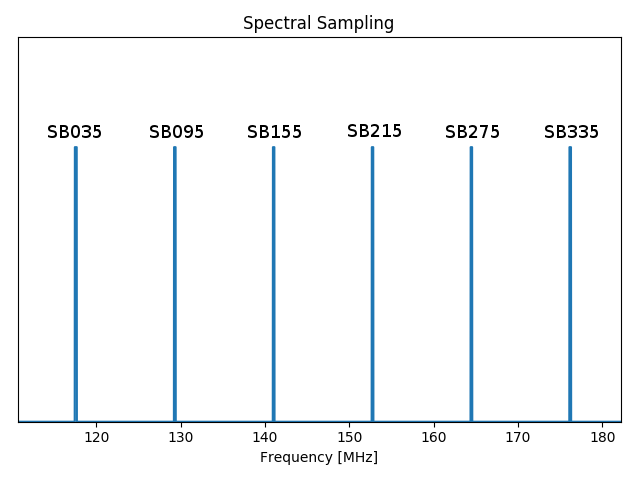
\includegraphics[width=0.5\textwidth]{images/FreqSampLabelled}
}{%
  \caption{\label{fig.freqsamp}Position of subbands chosen across full LOFAR bandwidth}%
}
\capbtabbox{%
  \begin{tabular}{|cc|} \hline
  Subband & $\nu_\mathrm{min} - \nu_\mathrm{max}$ \\ \hline
  SB035   &  117.45-117.69\\
  SB095   & 129.21-129.41\\
  SB155   & 140.93-141.12\\
  SB215   & 152.65-152.84\\
  SB275   & 164.37-164.56\\
  SB335   &  176.08-176.28 \\\hline
  \end{tabular}\vspace{1.2cm}
}{%
  \caption{Frequency bounds for the subbands chosen}%
}
\end{floatrow}
\end{figure}

\pg
Because no high-resolution models exist for 3C295 at our observing frequencies, which span quite a large bandwidth, care must be taken not to bias our model in an unphysical direction. We acquire the initial calibration model by extracting features from a NASA/IPAC Extragalactic Database\footnote{\hyperref[here]{https://ned.ipac.caltech.edu/}} image of 3C295 \citepads[see][]{1991AJ....101.1623P}, shown in Fig. \ref{fig.vla.3c295}. This feature extraction is carried out using PyBDSM \citepads{2015ascl.soft02007M}, changing all extracted Gaussians into points\footnote{This practice ensures that wrongly-estimated Gaussians do not end up introducing unphysical bias during calibration.}.
\begin{figure}[h]
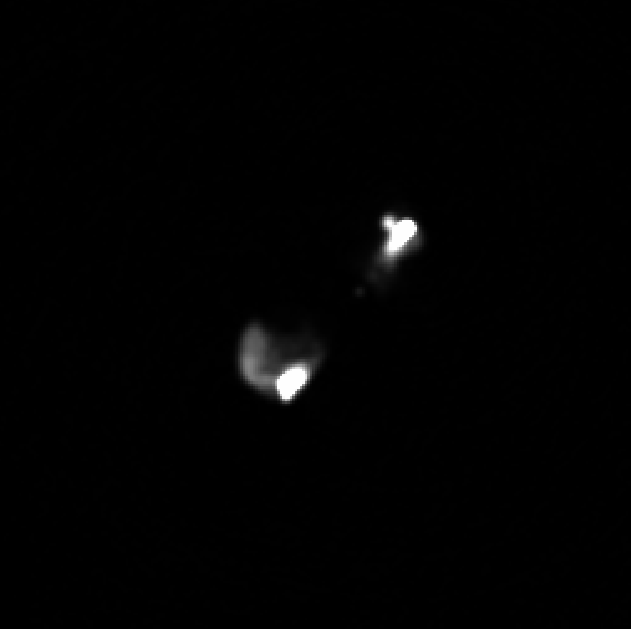
\includegraphics[width=0.4\linewidth]{images/3c295-vla}
\caption{\label{fig.vla.3c295}VLA observation of 3C295 at 8.7 GHz. Pixel size is $0.2''$.}
\end{figure}

\pg
For SB035, the gain curves for all antenna when calibrating with the initial model are as shown in Fig \ref{fig.sb035.gains.pass1}. Note that, especially for the international baselines, the gain amplitudes show a lot of structure: this is unphysical, and represents the unmodelled flux being absorbed into the gain solutions.
\begin{figure}[h!]
\includegraphics[width=0.9\linewidth]{images/{SB035.gains.pass1}.png}
\caption{\label{fig.sb035.gains.pass1} Gain curves for four LOFAR stations in SB035. Calibration was done using the VLA model. The blue curve shows the gain amplitude, while the green curve shows the phase. Here, only the values for the XX correlation are shown; they are indicative of the other Jones term properties.}
\end{figure}

\pg
A few features are immediately visible in Fig. \ref{fig.sb035.gains.pass1}. Firstly, we see in the gain amplitude curves of the core and remote stations that the gains for the last 2 hours of observation are noisier than the rest. This behaviour can be seen for most core and remote stations. Thankfully, the quality-based weighting schemes ought to optimise the contribution from these noisy visibilities, and so this is not too concerning. We see that the amplitude curves for the core and remote stations are nice and flat, with little structure to be seen: this is very encouraging, as this is what we expect "physical" gain curves to look like. In other words, we see little pollution from unmodelled sources in the calibration model for core and remote stations. The phase seems reasonable, with some structure but not dominated by noise. Note that the phase is expected to wrap from $-\pi$ to $\pi$ and vice-versa, which is what the fast oscillations in the last half of the phase gains of RS407HBA correspond to.

\pg
As for the international station gains, we see the presence of structure in the amplitude gain curve. This is indicative of the presence of sky model errors, which is expected: this is, after all, the gain curves after the first pass of calibration (i.e. without self-calibration). Very little information can be extracted from the phase curves, which wrap very fast: this is expected behaviour, as longer baselines rotate faster than shorter ones.

\pg
As calibration improves, however, we expect to get more of the true sky in our model. This, in turn, ought to decrease the structure in the gain curves. Fig \ref{fig.sb035.gains.pass4} shows the gain curves for the same antennas after 3 passes of self-calibration.
\begin{figure}[h!]
\includegraphics[width=0.9\linewidth]{images/{SB035.gains.pass4}.png}
\caption{\label{fig.sb035.gains.pass4} Gain curves for four LOFAR stations in SB035 after 3 passes of self-calibration. The blue curve shows the gain amplitude, while the green curve shows the phase. Here, only the values for the XX correlation are shown; they are indicative of the other Jones term properties.}
\end{figure}

\pg
As we can see, the last two hours remain noisy compared to the first two. What is interesting here is the evolution of the amplitude gain curves for DE602HBA and SE607HBA; while there is clearly still structure in the amplitude curves, we see that some of the structure is no longer present in the curves. What this indicates is that the sky model has improved compared to what it had been, but there is still room for improvement: indeed, this is as expected, as there are many more sources than 3C295 within the primary beam. 

\pg
This self-calibration was performed over all 6 subbands simultaneously; this allowed us to constrain the flux distribution in the sky as a function of frequency, even though the absolute scale in each image is known to be wrong. The absolute scale distribution being wrong is no issue, however; indeed, for each given subband, the gains are all wrong by the same multiplicative factor. This factor changes between subbands, however, and so the corrected visibilities must be corrected by the appropriate multiplicative factor for the true position-dependent spectral indices to be found. Mathematically, we have:
%A_\mathrm{true}(\nu) 
\begin{align}
\mathbf{V}_{pq}^\mathrm{corr.}(t,\nu) &= (a_\mathrm{false}(\nu) \mathbf{\tilde{G}}_{p,t}^{\nu})^{-1}{\mathbf{V}_{pq}^\mathrm{meas.}(t,\nu) }{(a_\mathrm{false}(\nu) \mathbf{\tilde{G}}^{\nu})^{-1}}\\
\mathbf{V}_{pq}^\mathrm{meas.}(t,\nu) &=(a_\mathrm{true}(\nu) \mathbf{{G}}_{p,t}^{\nu}) \mathbf{X}_{pq}(t,\nu) (a_\mathrm{true}(\nu) \mathbf{{G}}_{p,t}^{\nu}) %}{(a_\mathrm{false}(\nu) \mathbf{\tilde{G}}_{p,t}^{\nu})(a_\mathrm{false}(\nu) \mathbf{\tilde{G}}_{q,t}^{\nu})}
\end{align}
where uppercase, boldface letters denote $2\times 2$ Jones matrices, and lowercase letters are scalars. Here, $a_\mathrm{false}(\nu)$ is the incorrect scaling factor applied at frequency $\nu$ by calibrating without the proper spectral indices for all the components of 3C295, while $a_\mathrm{true}(\nu)$ is the correct scaling factor. The true scaling factor is known from low-resolution calibrator analysis, while the false scaling factor is an arbitrary function of frequency.
Assuming that our estimate for the Jones matrices is accurate (modulo the scaling factor), i.e. that $\mathbf{\tilde{G}}_{q,t}^{\nu}\approx \mathbf{{G}}_{q,t}^{\nu}$, then 
\begin{align}
(a_\mathrm{false}(\nu) \mathbf{\tilde{G}}_{p,t}^{\nu})^{-1}(a_\mathrm{true}(\nu) \mathbf{{G}}_{p,t}^{\nu}) &= \frac{a_\mathrm{false}(\nu)}{a_\mathrm{true}(\nu)} (\mathbf{\tilde{G}}_{p,t}^{\nu})^{-1}\mathbf{{G}}_{p,t}^{\nu}\\
&\approx \frac{a_\mathrm{false}(\nu)}{a_\mathrm{true}(\nu)} \I
\end{align}
and so
\begin{align}
\mathbf{V}_{pq}^\mathrm{corr.}(t,\nu) &\approx  \left(\frac{a_\mathrm{false}(\nu)}{a_\mathrm{true}(\nu)}\right)^2\mathbf{X}_{pq}(t,\nu)
\end{align}
we can thus recover the properly-scaled visibilities in each subband by normalising the visibilities (i.e. divide by whatever $a_\mathrm{false}$ happens to be with a given calibration at a given frequency) and subsequently scaling them by $a_\mathrm{true}$ so that the average value in the corrected visibilities is equal to what's expected at this frequency.

\pg
Having calibrated our 6 subbands with the VLA model, we deconvolve them simultaneously. This allows us to improve the conditioning of the imaging inverse problem. After three passes of self-calibration, we have a spectral cube with 6 frequency slices centred on the various subbands. The stacked residual images are in Fig \ref{fig.3c295.stack.selfcal.uvcut}, before and after self-calibration. We see that noise falls by a factor of [?].
\begin{figure}[h!]
\centering
\begin{subfigure}{.43\textwidth}
\resizebox{\hsize}{!}{\includegraphics{images/{VLApybdsmModel.FullBW.automate.sc.pass1.app.restored.normalised.fits}.png}}
\caption{\label{fig.3c295.stack.selfcal.uvcut.SC1} Calibrated with the VLA model: there is quite a bit of noise.}
\end{subfigure}
\hfill
\begin{subfigure}{.43\textwidth}
\resizebox{\hsize}{!}{\includegraphics{images/{VLApybdsmModel.FullBW.automate.sc.pass4.app.restored.normalised.fits}.png}}
\caption{\label{fig.3c295.stack.selfcal.uvcut.SC3} Same data after 3 passes of self-calibration: the noise is decreased.}
\end{subfigure}
\caption{\label{fig.3c295.stack.selfcal.uvcut} Images made with 6 subbands spread across the LOFAR bandwidth.}
\end{figure}
The frequency-dependent model is shown in Fig. [ref]
\pg
               !!! SHOW GAIN CURVES, LOTS OF PLOTS ETC
\pg
               !!! ANALYSE CONVERGENCE OF CALIBRATION ACROSS SUBBANDS
\pg
apply beam to account for different sensitivities of different baselines
\pg
use full-Jones solver (i.e. solve for a 2x2 complex matrix) to account for effects such as Faraday rotation etc
\pg
!!! SHOW JONES CHAIN WE SOLVE FOR AND EXPLAIN IT, MATHS ETC: $\mat{B}\mat{J}$ for Beam*Jones
\pg
!!! SHOW DIRECTION-DEPENDENT PSF EFFECT WHICH WE MODEL


% % % % % % % % % % % % % % % % % % % % % % %
\section{Overlays \& Spectral Analaysis}

\subsection{Overlays of 3C295 at Multiple Frequencies}
\pg
Show overlays of our low-freq model onto images of 3c295 at various other freqs - VLA, optical, IR, X-ray, etc.

\pg
Comment on behaviour of various components, astrometric accuracy, etc

\subsection{Spectral Analaysis}

\pg
Work with Astron guy to extract spectral behaviour of various components of 3C295 over multiple wavelengths, since he's got a purpose-built package